\tikzsetnextfilename{images/scaling_test_problem_geometry_pdf}
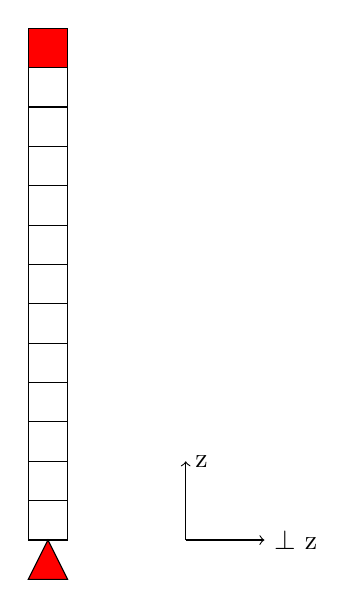
\begin{tikzpicture}
\foreach \x in {1,..., 12} \draw(0, 0.5*\x-0.5) rectangle +(.5,.5);
\filldraw[fill=red] (0, 6) rectangle +(.5,.5); 
\filldraw[fill=red] (0, -0.5) -- (0.25, 0) -- (0.5, -0.5) -- cycle;
\draw[->] (2,0) -- (2, 1) node[anchor=west] {z};
\draw[->] (2,0) -- (3, 0) node[anchor=west] {$\perp$ z};
\end{tikzpicture}